\chapter{Table des pages}
\label{annexe:memory_page_table}

%\section{Table des pages Intel}


\begin{figure}[H]
    \center
    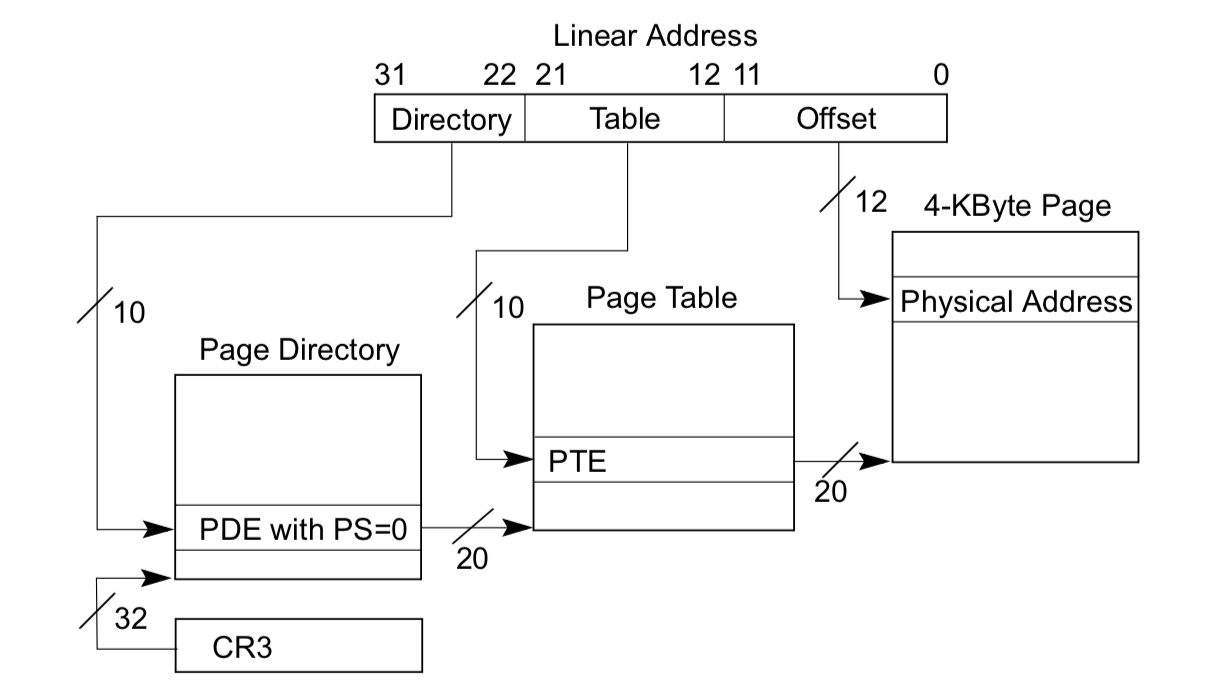
\includegraphics[width=10cm]{images/memory_page_table_32bits.png}
    \caption{\label{pic:memory_page_table_32bits} Table de pages utilisant 32 bits de l'adresse virtuelle dans une table à 3 niveaux \cite{intel64and}}.
\end{figure}

\begin{figure}
    \center
    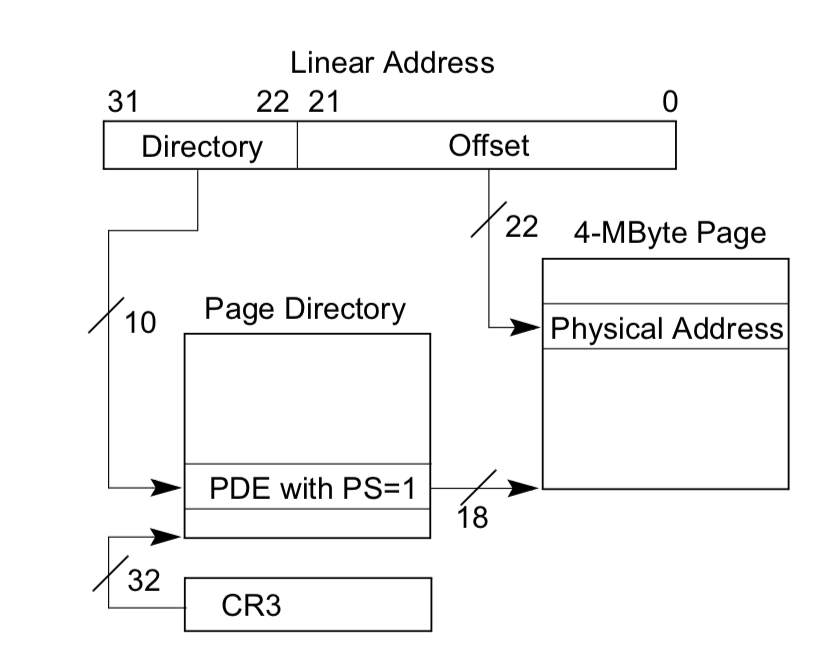
\includegraphics[width=10cm]{images/memory_page_table_32bits_large.png}
    \caption{\label{pic:memory_page_table_32bits_large} Table de pages pour des page large de 2 MiB\cite{intel64and}}.
\end{figure}


\begin{figure}
    \center
    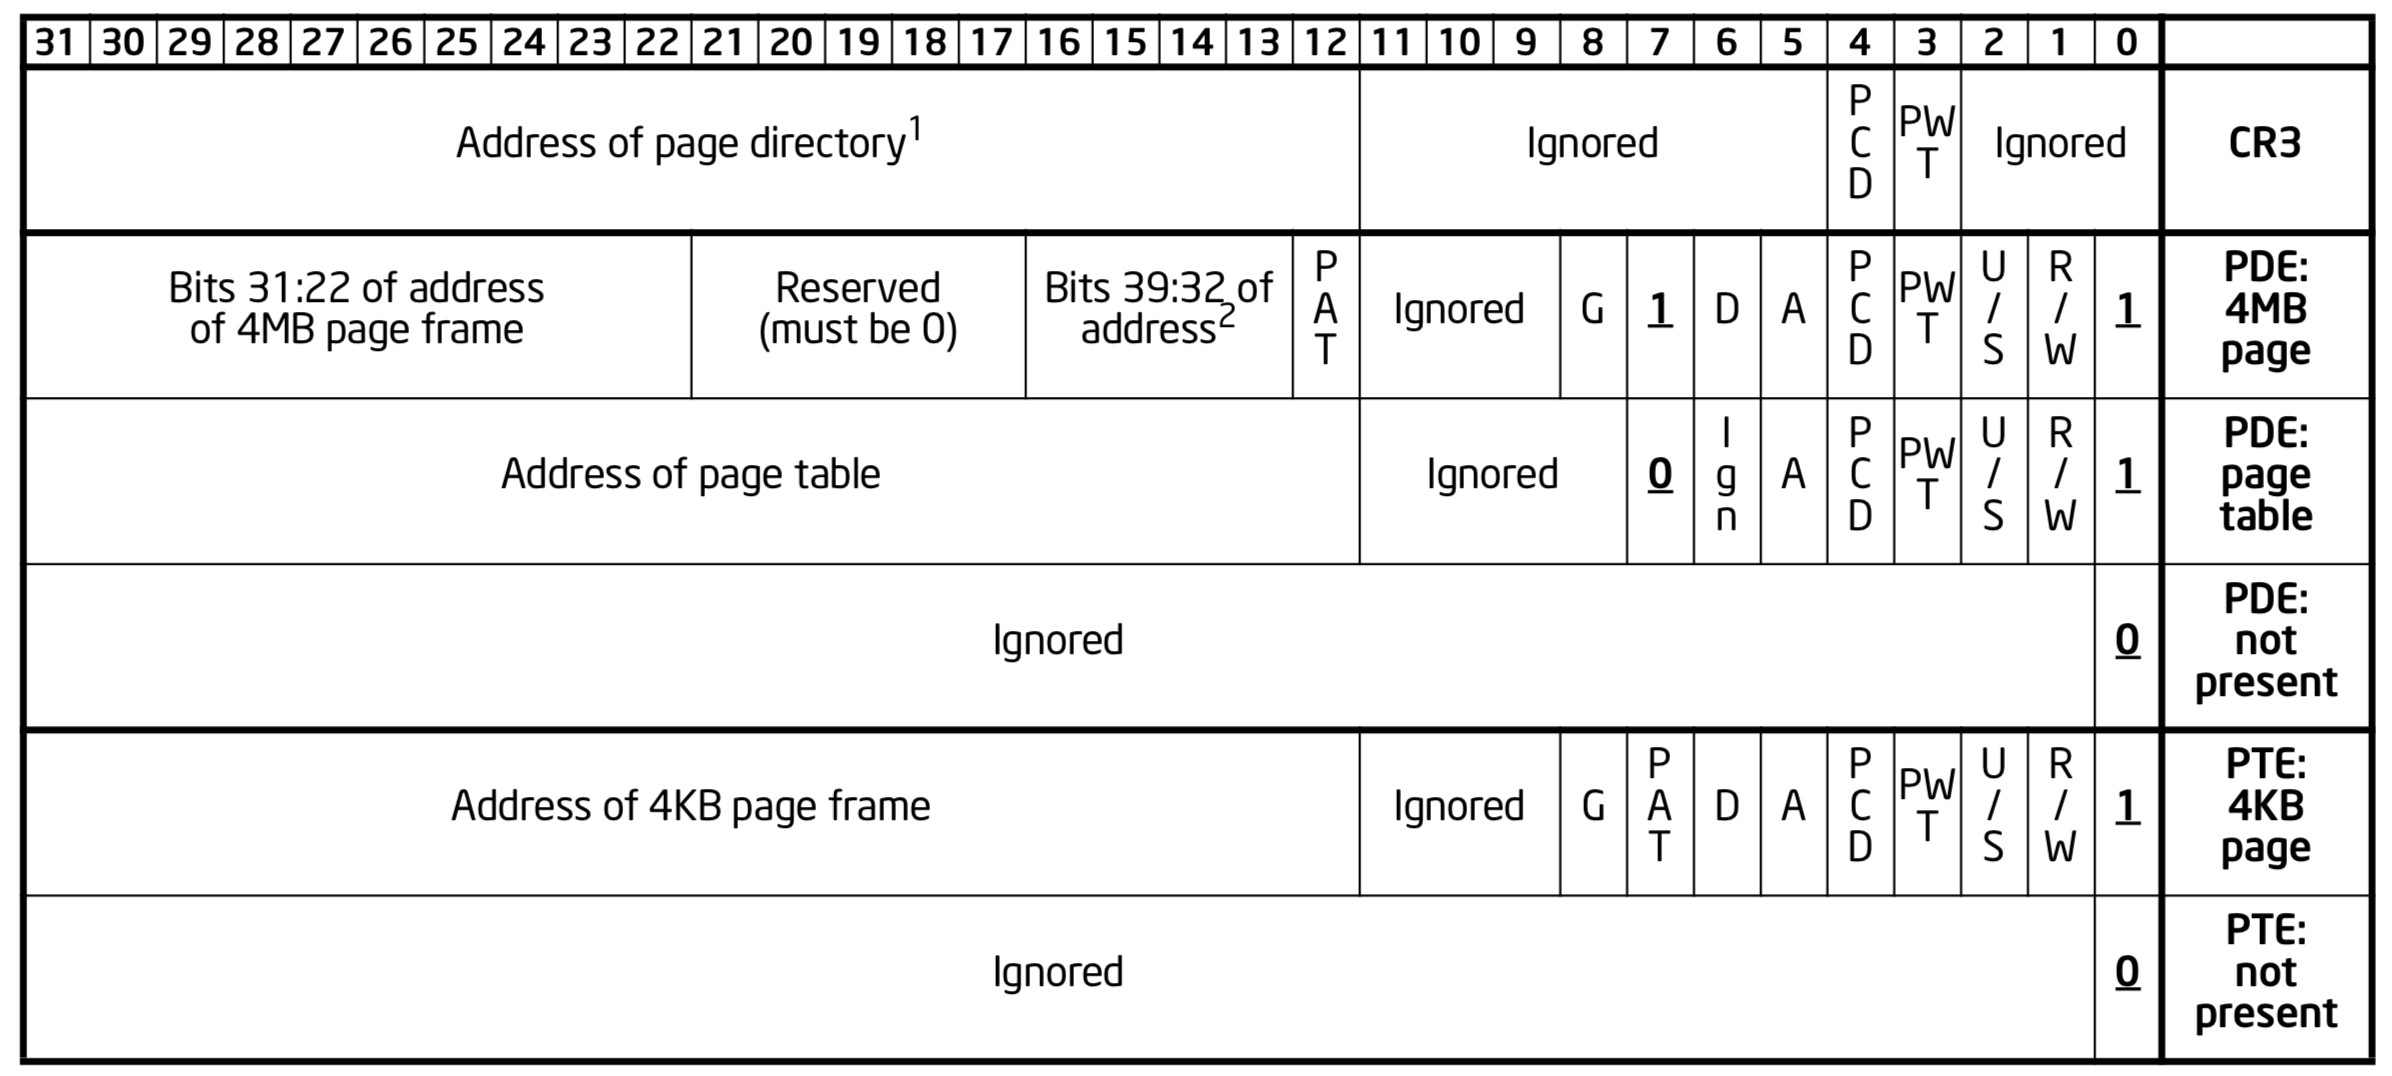
\includegraphics[width=10cm]{images/memory_page_table_entry_intel.png}
    \caption{\label{pic:memory_page_table_entry_intel} Structure d'une entrée dans la table de page \cite{intel64and}}.
\end{figure}



%\begin{figure}[p]
  %\centering
  %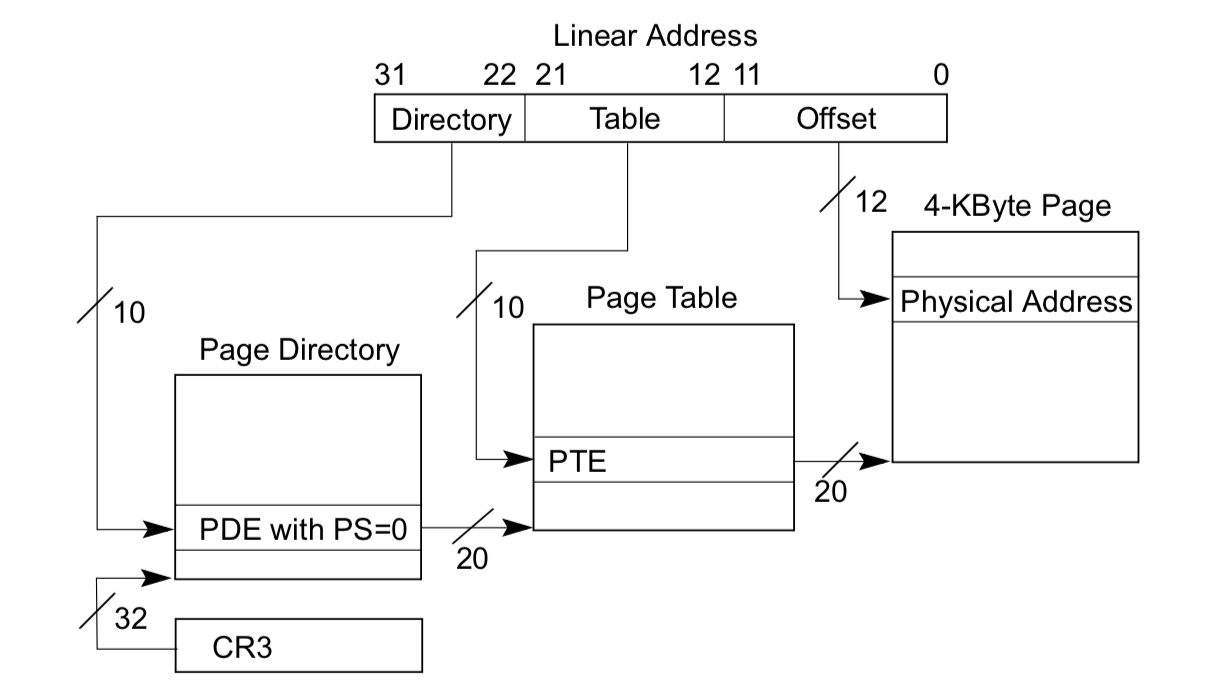
\includegraphics[width=0.2\textwidth]{images/memory_page_table_32bits.png}
  %\caption{Capt1.}
  %\label{fig:lab1}
  %\centering
  %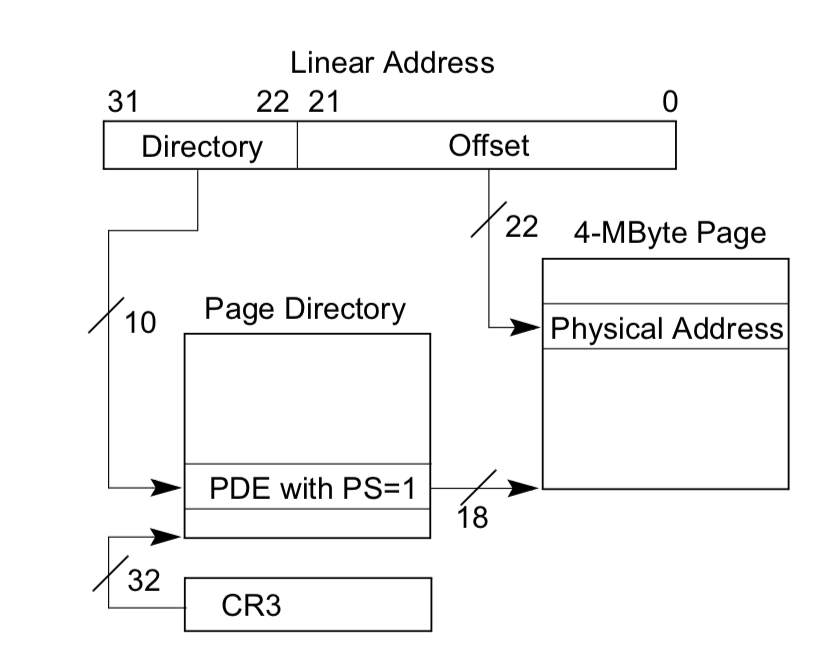
\includegraphics[width=0.2\textwidth]{images/memory_page_table_32bits_large.%png}
  %\caption{Capt2.}
  %\label{fig:lab2}
  %\centering
  %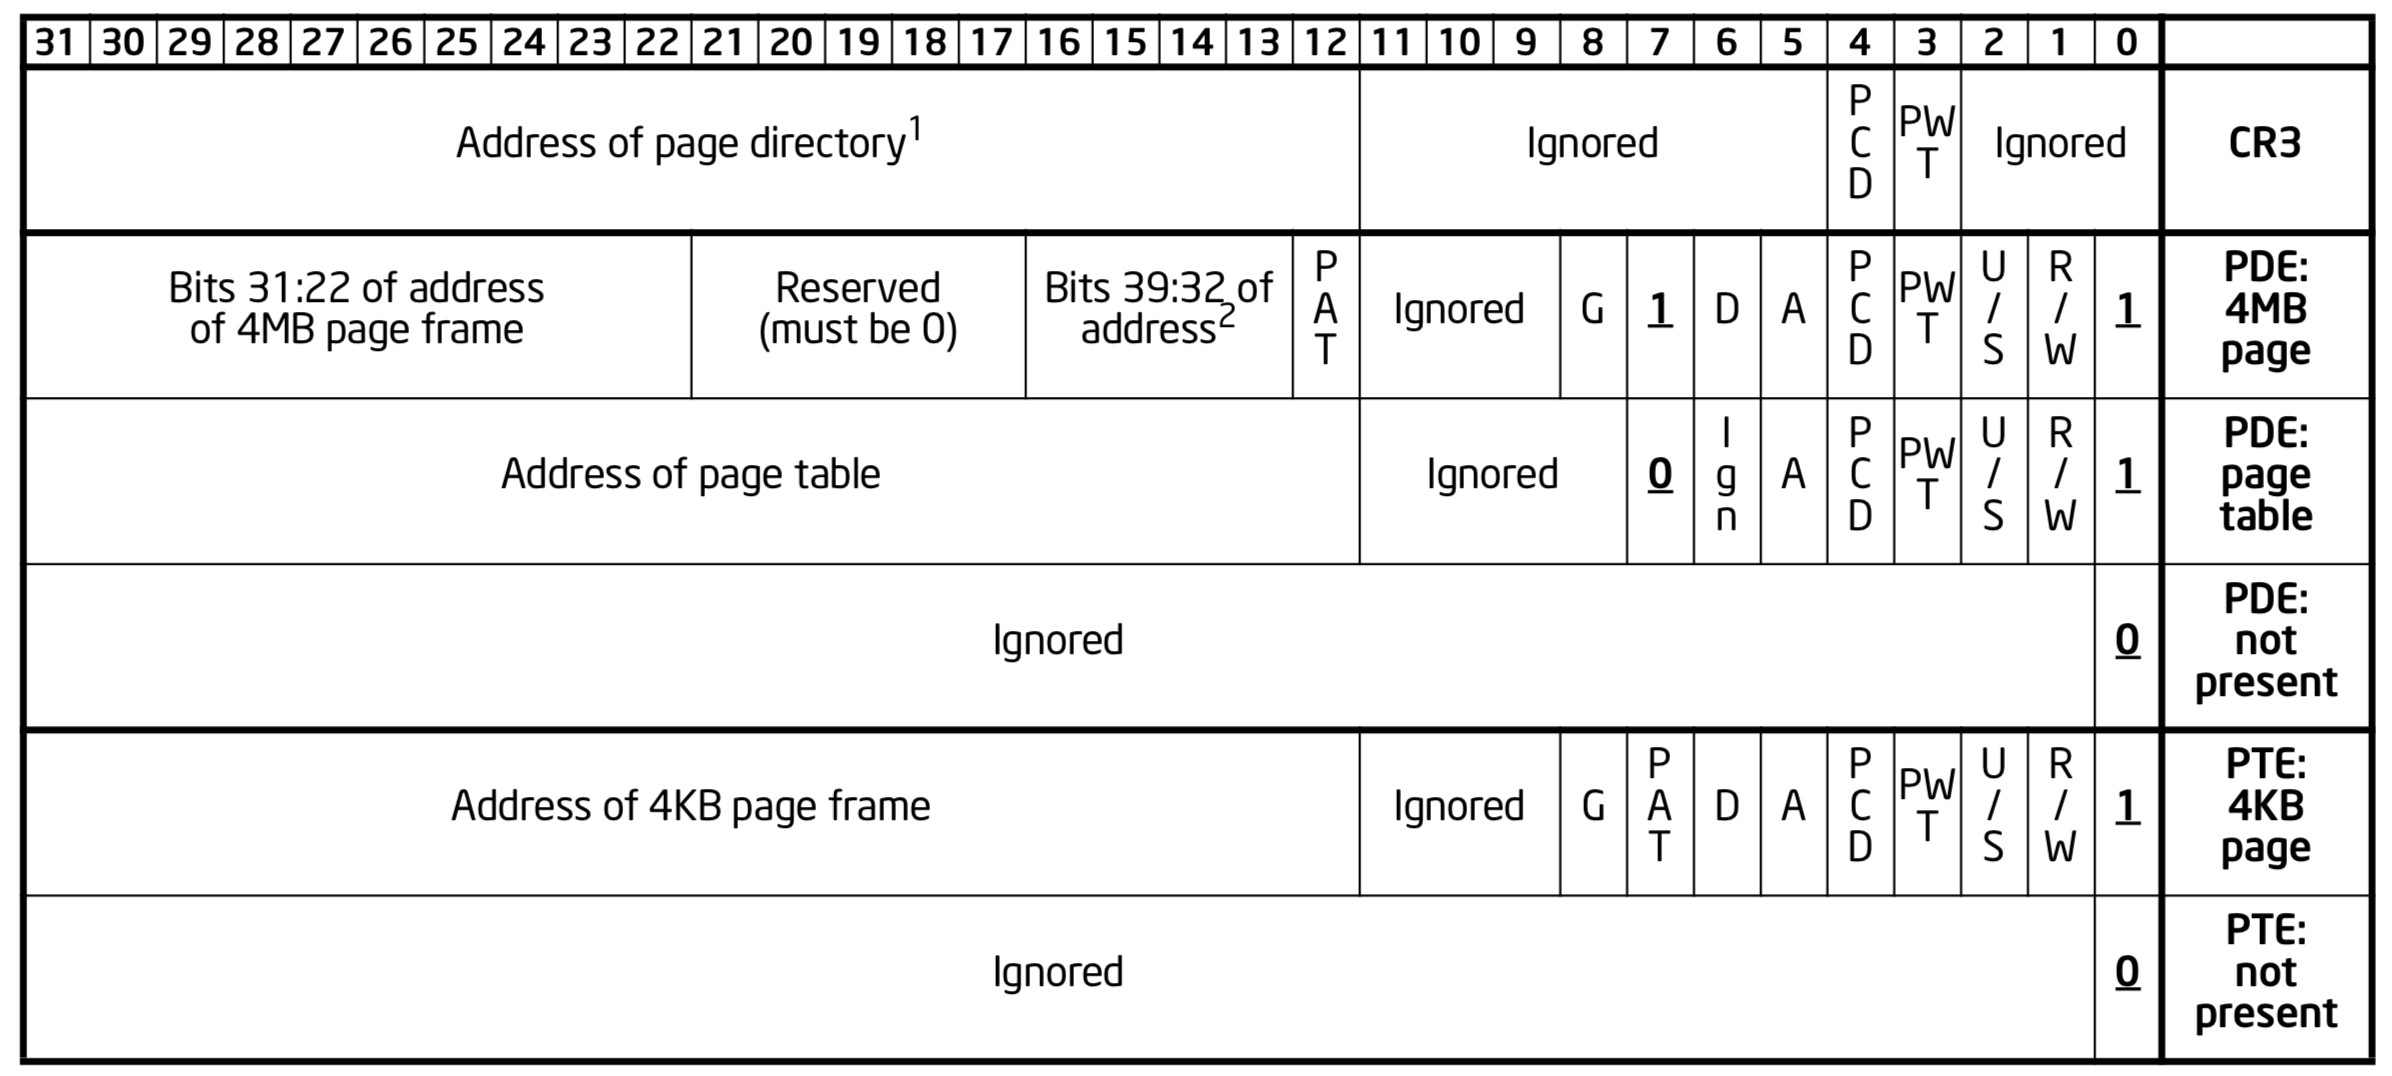
\includegraphics[width=0.2\textwidth]{images/memory_page_table_entry_intel.p%ng}
  %\caption{capt3.}
  %\label{fig:lab3}
%\end{figure}